%!TEX root = ../Hardtung_PP_WiSe1920.tex

\section{Program Features and Use}
\label{program}

The structure of the developed origami diagramming program (ff. \gls{origrammer}) follows a similar approach to the real life diagramming process. To create a new model, we start with some general decisions. When selecting the ``File > New'' menu item, a new dialog box opens (see Figure \ref{fig:newModel}) where \emph{paper shape, size} and the \emph{paper color} of both sides can be specified. Additionally, the text fields \emph{Title, Author, Comments} can be filled out to provide further information of the model. These options can also be accessed and changed during the diagramming process (except for the paper shape) when selecting ``Edit > Model Preferences''.
\begin{figure}[htbp]
	\centering
	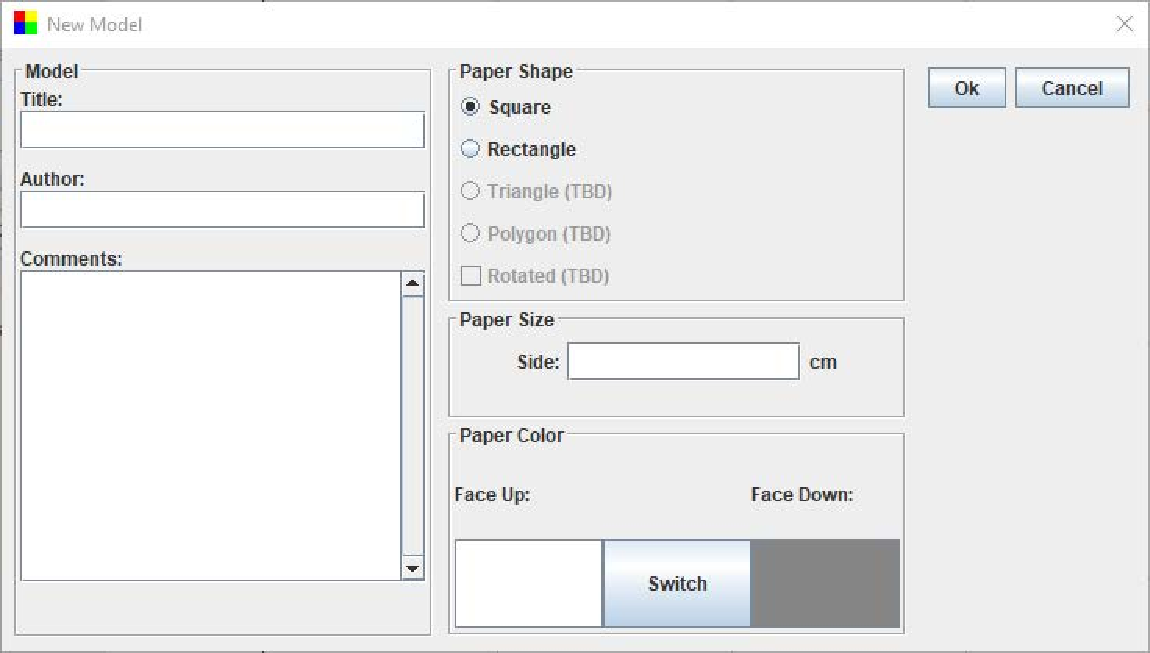
\includegraphics[width=0.7\textwidth]{newModel}
	\caption{New Model dialog box}
	\label{fig:newModel}
\end{figure}\\
After specifying all the model settings, the main diagramming window is presented to the user (see Figure \ref{fig:origrammerMain}). This main editing area consists of four segments:

\subsubsection*{Side Panel}
On the left side of the main window the side panel is located. It presents the toolbar where the user can switch between inputting lines, arrows, general origami symbols, the selection tool (further explained later), a measurement tool, as well as a filling tool. Furthermore, a helping grid can be displayed and adjusted to ease the input of lines. Additionally, when requiring more clarity during the diagramming process, the faces that got filled with the filling tool as well as all vertices can be turned invisible.

\subsubsection*{Top Panel}
The top panel is directly connected to the side panel, as it shows the actual settings, depending on what tool from the toolbar is active. Such as for the Line Input Tool, the top panel displays a combo box that contains the previously mentioned six different arrow types of origami. For other active tools this panel can show scaling or rotating options, different combo boxes, text fields or check boxes for a variety of adjustments.

\subsubsection*{Navigation Panel}
Unlike the aforementioned panels, the navigation panel directly influences the model panel. As the name already states, this panel allows the navigation through the individual diagram steps. It also provides a text field to give the textual instructions for the current step. Furthermore different options can be selected on what should happen when a new step is created. The user can either create an empty step, copy the previous step or create a step with the basic paper shape that got defined in the \emph{Model Preferences}.

\subsubsection*{Model Panel}
The previously specified piece of paper is displayed in the model panel. This is the main editing area where the paper, together with the arrows and other symbols, is rendered to represent the current state of the paper for each folding step.
\begin{figure}[htbp]
	\centering
	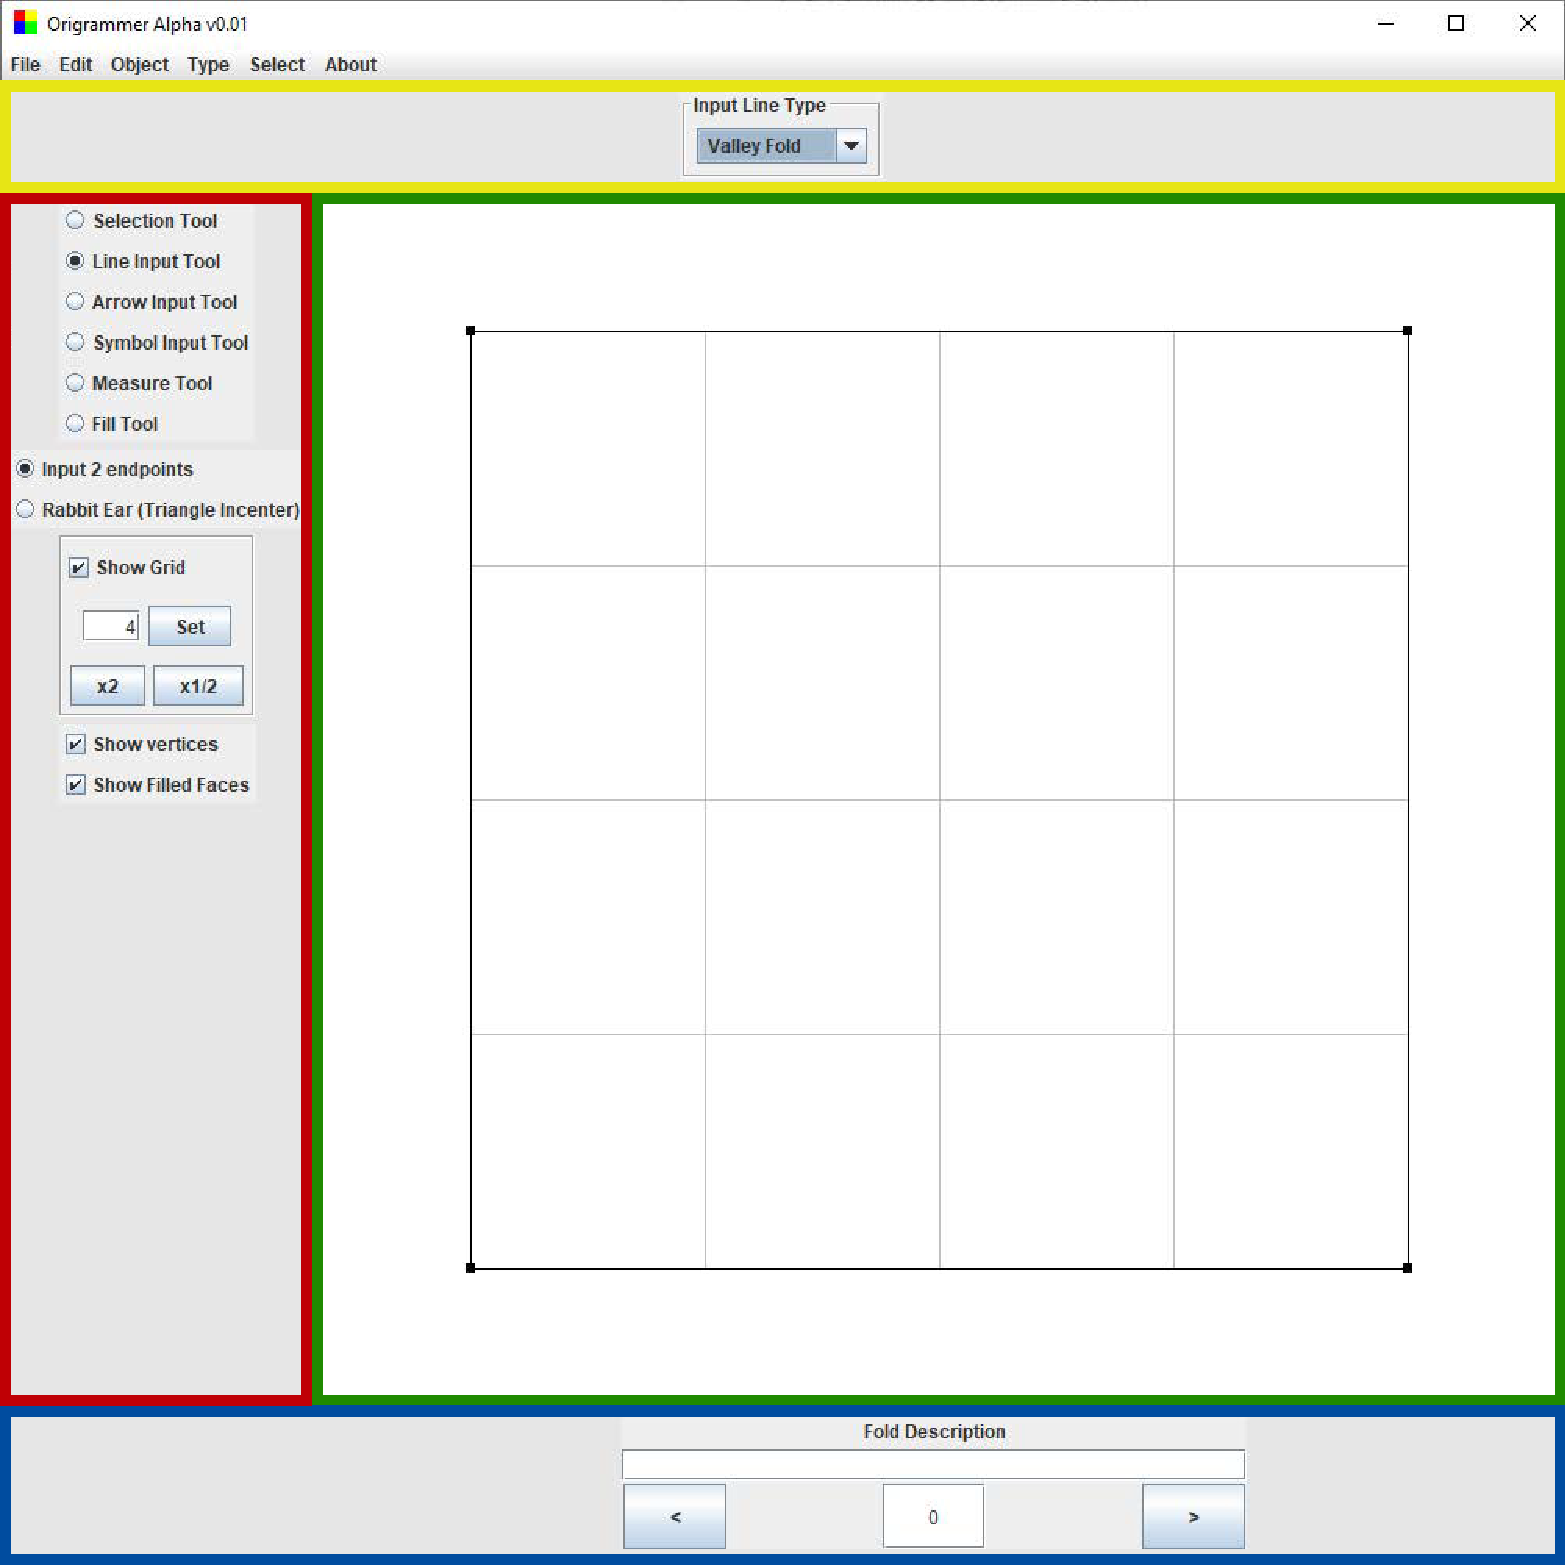
\includegraphics[width=1\textwidth]{OrigrammerMainParts}
	\caption{Origrammer main window \emph{(Yellow = Top Panel; Red = Side Panel; Blue = Navigation Panel; Green = Main Panel)}}
	\label{fig:origrammerMain}
\end{figure}